\documentclass[11pt]{beamer}
\usetheme{CambridgeUS}
\usepackage[utf8]{inputenc}
\usepackage{amsmath}
\usepackage{amsfonts}
\usepackage{amssymb}
\usepackage{graphicx}
\usepackage{pgfpages}
\usepackage{framed}
\usepackage{xcolor}
\usepackage[most]{tcolorbox}
\usepackage{soul}
\usepackage{empheq}

\newcommand*{\itemimg}[1]{%
  \raisebox{-.3\baselineskip}{%
    \includegraphics[
      height=\baselineskip,
      width=\baselineskip,
      keepaspectratio,
    ]{#1}%
  }%
}

\newtcbox{\mymath}[1][]{%
    nobeforeafter, math upper, tcbox raise base,
    enhanced, colframe=blue!30!black,
    colback=blue!10, boxrule=1pt,
    #1}

\newcommand{\highlight}[1]{%
  \colorbox{yellow!100}{$\displaystyle#1$}}

\author{Giovanni Della Lunga\\{\footnotesize giovanni.dellalunga@unibo.it}}
%\title{1 - Introduction to Machine Learning}
%\title{2.1 - Data Pre-Processing}
\title{3.2 - Support Vector Machines}
%\title{4.2 - Decision Trees}
%\title{6 - Text Vectorization}
%\title{7 - Classification for Text Analysis}
%\title{8 - Clustering for Text Similarity}
%\title{9 - Information Extraction}
\subtitle{} % (optional)
\setbeamercovered{transparent} 
%\institute{Introduction to Machine Learning for Finance} 
\date{Bologna - February-April, 2025} 

\begin{document}

\begin{frame}
\titlepage
\end{frame}

\AtBeginSection[]
{
%	\begin{frame}<beamer>
%  		\frametitle{Outline}
%  		\tableofcontents[currentsection]
%	\end{frame}
  	\begin{frame}
  		\vfill
  		\centering
  		\begin{beamercolorbox}	[sep=8pt,center,shadow=true,rounded=true]{title}  		\usebeamerfont{title}\insertsectionhead\par%
  		\end{beamercolorbox}
  		\vfill
  \end{frame}
}
\AtBeginSubsection{\frame{\subsectionpage}}





\section{Introduction}
%..................................................................
\begin{frame}{Linear Separation}
\begin{columns}[T] % align columns
\begin{column}{.48\textwidth}
        \begin{itemize}
		\item \textbf{Linearly Separable Data points}: Data points can be said to be linearly separable if a separating boundary/hyperplane can easily be drawn showing distinctively the different class groups. 
		\item Linear separable data points mostly require linear machine learning classifiers such as Logistic regression for example.
        \end{itemize}
\end{column}%
\hfill%
\begin{column}{.48\textwidth}
    %\fbox{
        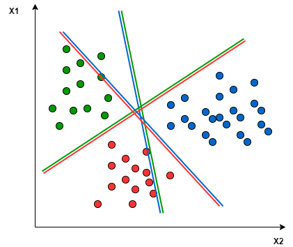
\includegraphics[width=\linewidth]{../5-pictures/chapter-4-4_pic_0.png}
    %}
\end{column}%
\end{columns}
\end{frame}
%..................................................................
\begin{frame}{Linear Separation}
	\begin{center}
	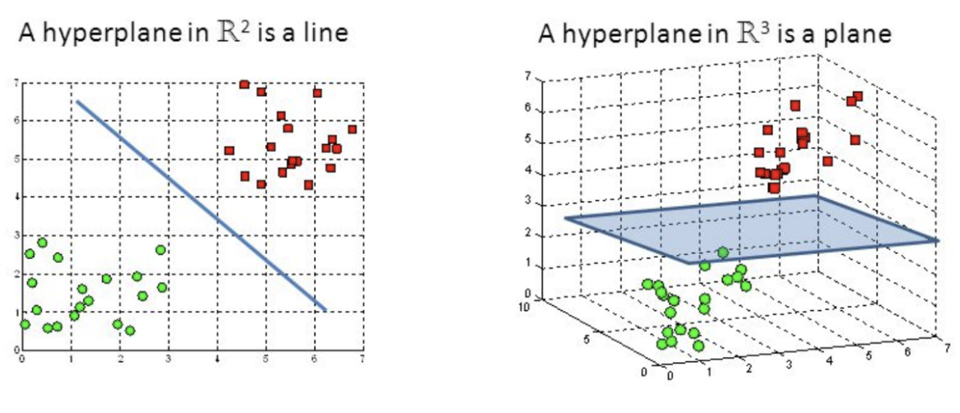
\includegraphics[scale=0.4]{../5-pictures/chapter-4-4_pic_1.png}
	\end{center}
\end{frame}

\section{Perceptron}
\begin{frame}{Perceptron Overview}
    \begin{itemize}
        \item Introduced by Frank Rosenblatt in 1958.
        \item Used for binary classification problems.
        \item A single-layer neural network with step activation.
    \end{itemize}
\end{frame}

\begin{frame}{Perceptron Structure}
    \begin{itemize}
        \item Inputs with associated weights.
        \item Weighted sum plus bias.
        \item Step function activation.
    \end{itemize}
    %\includegraphics[width=0.6\textwidth]{perceptron_structure.png}
\end{frame}

\begin{frame}{Mathematical Formulation}
    $$ y = \begin{cases} 1, & \text{if } \sum w_i x_i + b \geq 0 \\ 0, & \text{otherwise} \end{cases} $$
\end{frame}

\begin{frame}{Perceptron Learning Rule}
    \begin{itemize}
        \item Initialize weights and bias.
        \item Update rule: $ w_i \leftarrow w_i + \eta (y - \hat{y}) x_i $
        \item Bias update: $ b \leftarrow b + \eta (y - \hat{y}) $
    \end{itemize}
\end{frame}

\begin{frame}{Perceptron Convergence Theorem}
    \begin{itemize}
        \item The perceptron algorithm converges if the data is linearly separable.
        \item The number of updates is bounded by the margin of separation.
    \end{itemize}
\end{frame}

\section{Support Vector Machines (SVMs)}
\begin{frame}{What is an SVM?}
    \begin{itemize}
        \item A powerful classification model.
        \item Finds the optimal separating hyperplane.
        \item Maximizes the margin between classes.
    \end{itemize}
\end{frame}

\begin{frame}{Mathematical Definition}
    $$ \min \frac{1}{2} ||w||^2 \quad \text{subject to } y_i (w \cdot x_i + b) \geq 1 $$
\end{frame}

\begin{frame}{Support Vectors and Margins}
    \begin{itemize}
        \item Support vectors are closest to the decision boundary.
        \item The margin is the distance between these points and the hyperplane.
    \end{itemize}
    %\includegraphics[width=0.6\textwidth]{svm_margin.png}
\end{frame}

\begin{frame}{Hard vs Soft Margin SVM}
    \begin{itemize}
        \item Hard Margin: No misclassification allowed.
        \item Soft Margin: Allows some misclassification to improve generalization.
    \end{itemize}
\end{frame}

\section{Kernel Methods}
\begin{frame}{The Kernel Trick}
    \begin{itemize}
        \item Maps data to a higher-dimensional space.
        \item Avoids explicit computation of feature transformation.
        \item Enables SVMs to work with non-linearly separable data.
    \end{itemize}
\end{frame}

\begin{frame}{Common Kernel Functions}
    \begin{itemize}
        \item Polynomial Kernel: $ K(x, y) = (x \cdot y + c)^d $
        \item Radial Basis Function (RBF) Kernel: $ K(x, y) = e^{-\gamma ||x - y||^2} $
    \end{itemize}
\end{frame}

\begin{frame}[fragile]{Example: RBF Kernel in Python}
    \textbf{Python Code:}
    \begin{verbatim}
    from sklearn.svm import SVC
    model = SVC(kernel='rbf', gamma=1)
    model.fit(X_train, y_train)
    \end{verbatim}
\end{frame}

\begin{frame}{Hyperparameter Tuning in SVMs}
    \begin{itemize}
        \item C: Controls trade-off between margin width and misclassification.
        \item Gamma: Defines influence of a single training example.
        \item Kernel Choice: Linear, Polynomial, RBF.
    \end{itemize}
\end{frame}

\end{document}
